\documentclass[fleqn,10pt]{wlscirep}
\usepackage[utf8]{inputenc}
\usepackage[T1]{fontenc}
\usepackage{lineno}
\linenumbers

\usepackage[figurename=Supplementary figure]{caption}
\usepackage{placeins}



\begin{document}
\begin{titlepage}
   \vspace*{\stretch{1.0}}
   \begin{center}
      \Large\textbf{Annotation guidelines for hard cases in CholecInstanceSeg}
   \end{center}
   \vspace*{\stretch{2.0}}
\end{titlepage}

\thispagestyle{empty}
\listoffigures
\newpage


% fluid
\begin{figure}[ht]
\centering
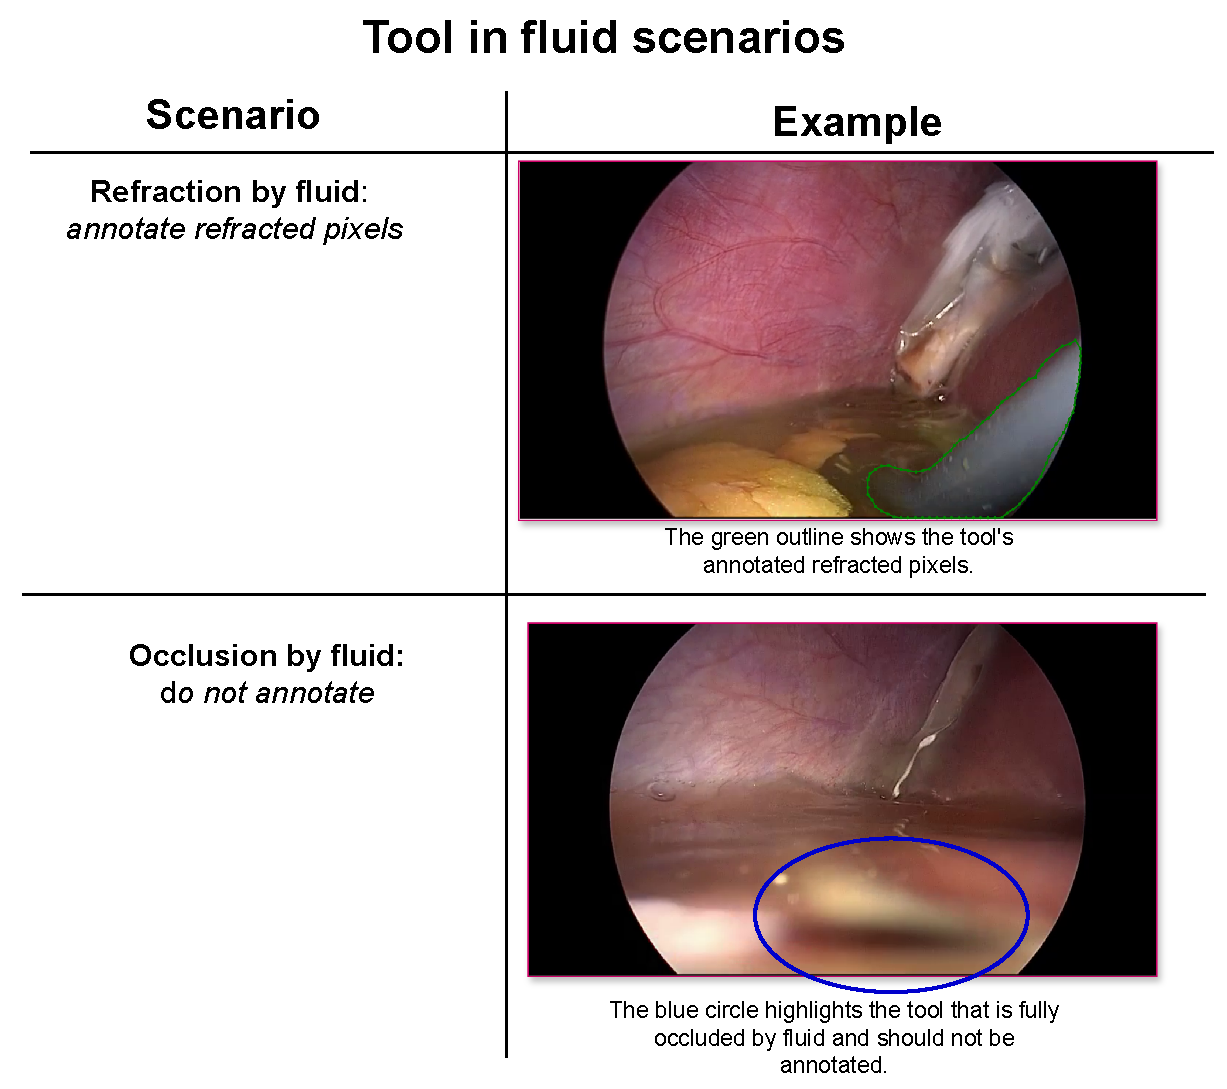
\includegraphics[width=0.9\linewidth]{imgs/hard_cases_annotating_instrument_in_fluid.pdf}
\caption{Annotation guidelines for tools in fluid scenarios}
\label{fig:fluid}
\end{figure}

\begin{figure}[ht]
\centering
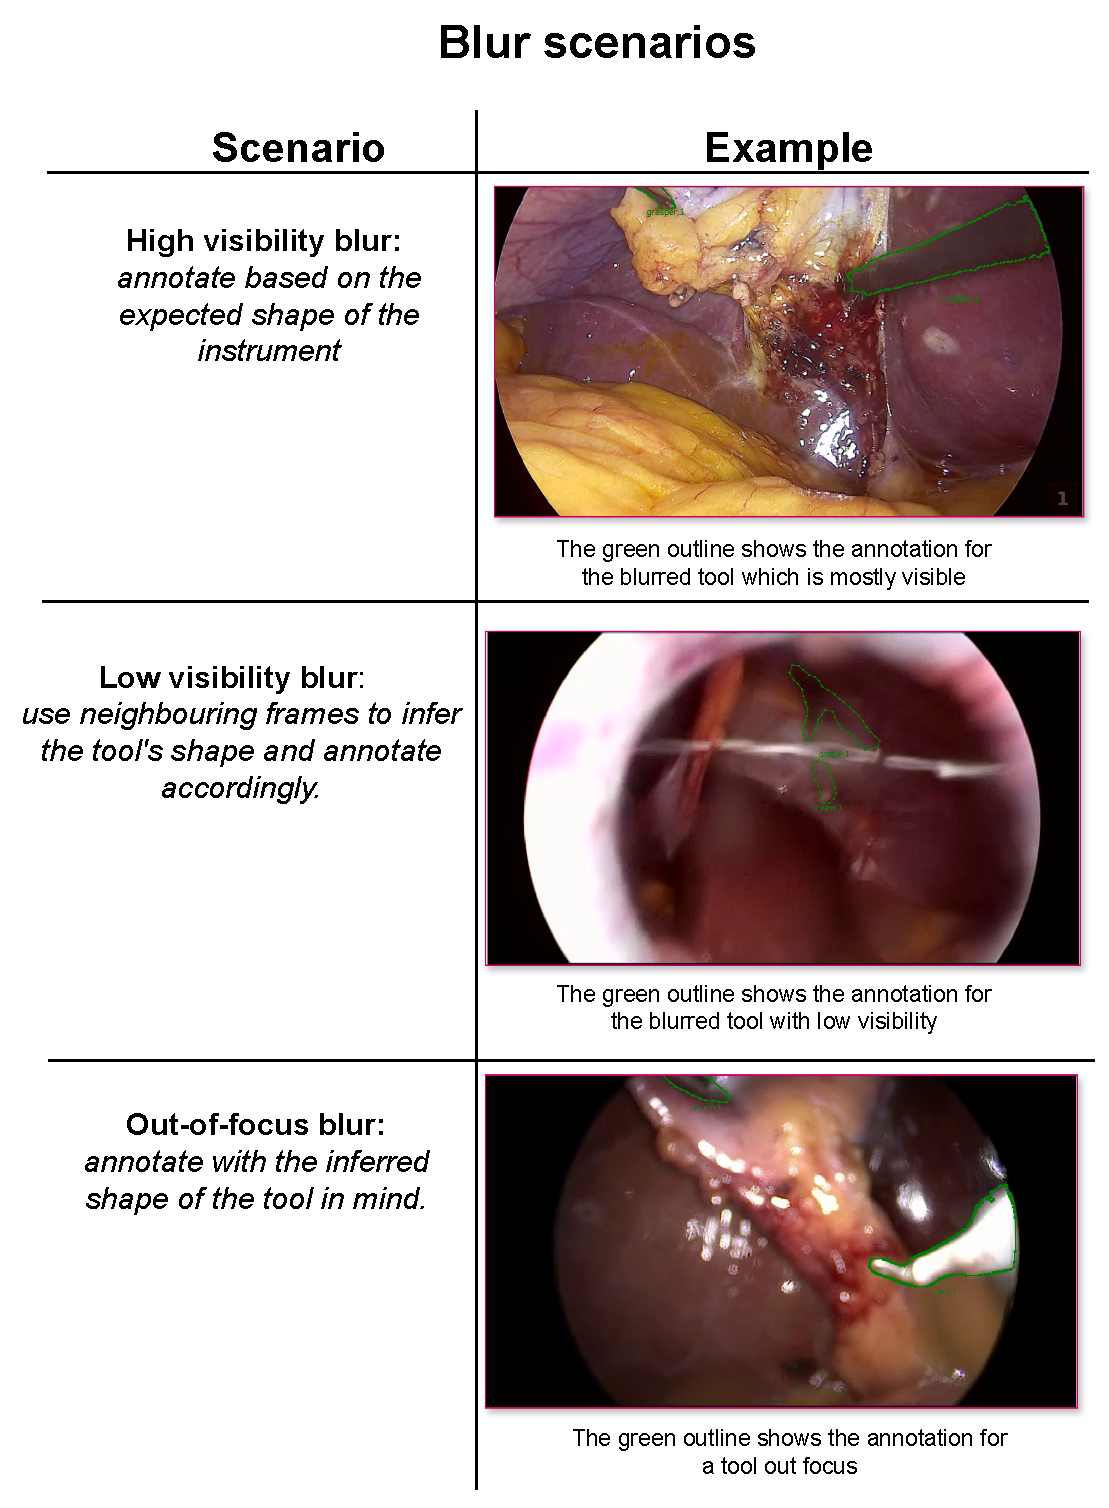
\includegraphics[width=0.9\linewidth]{imgs/hard_cases_blur.pdf}
\caption{Annotation guidelines for blur scenarios.}
\label{fig
}
\end{figure}

\begin{figure}[ht]
\centering
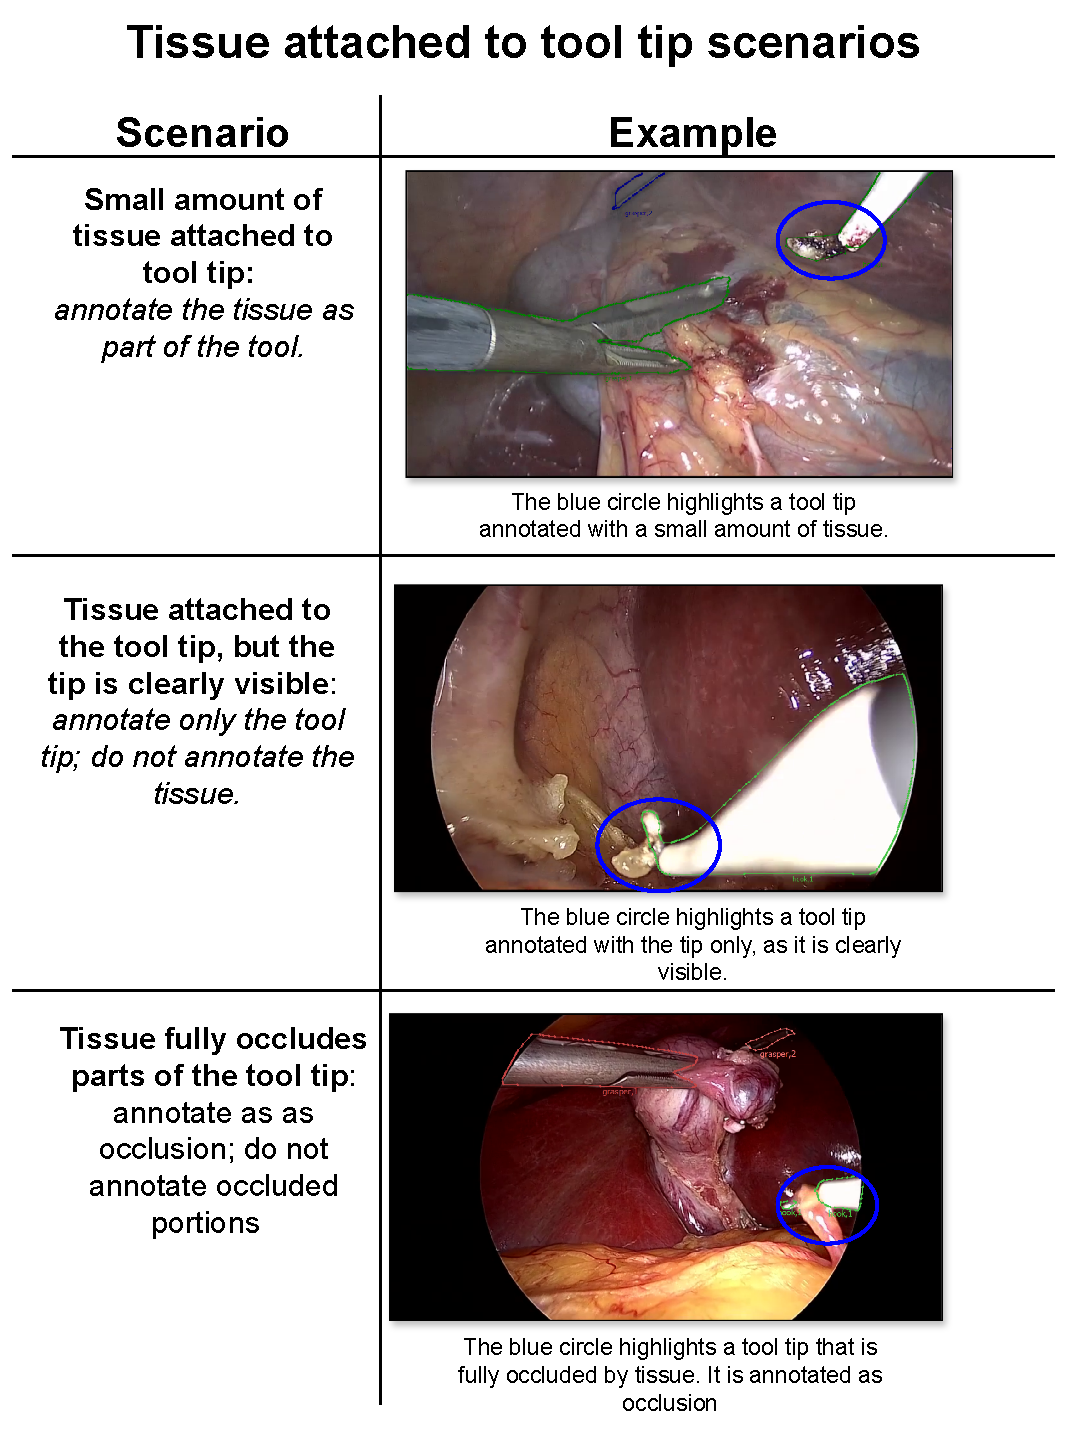
\includegraphics[width=0.9\linewidth]{imgs/hard_cases_attached_to_instrument.pdf}
\caption{Annotation guidelines for tissue attached to tool tip scenarios. }
\label{fig:tissue_tool_tip}
\end{figure}

\begin{figure}[ht]
  \centering
  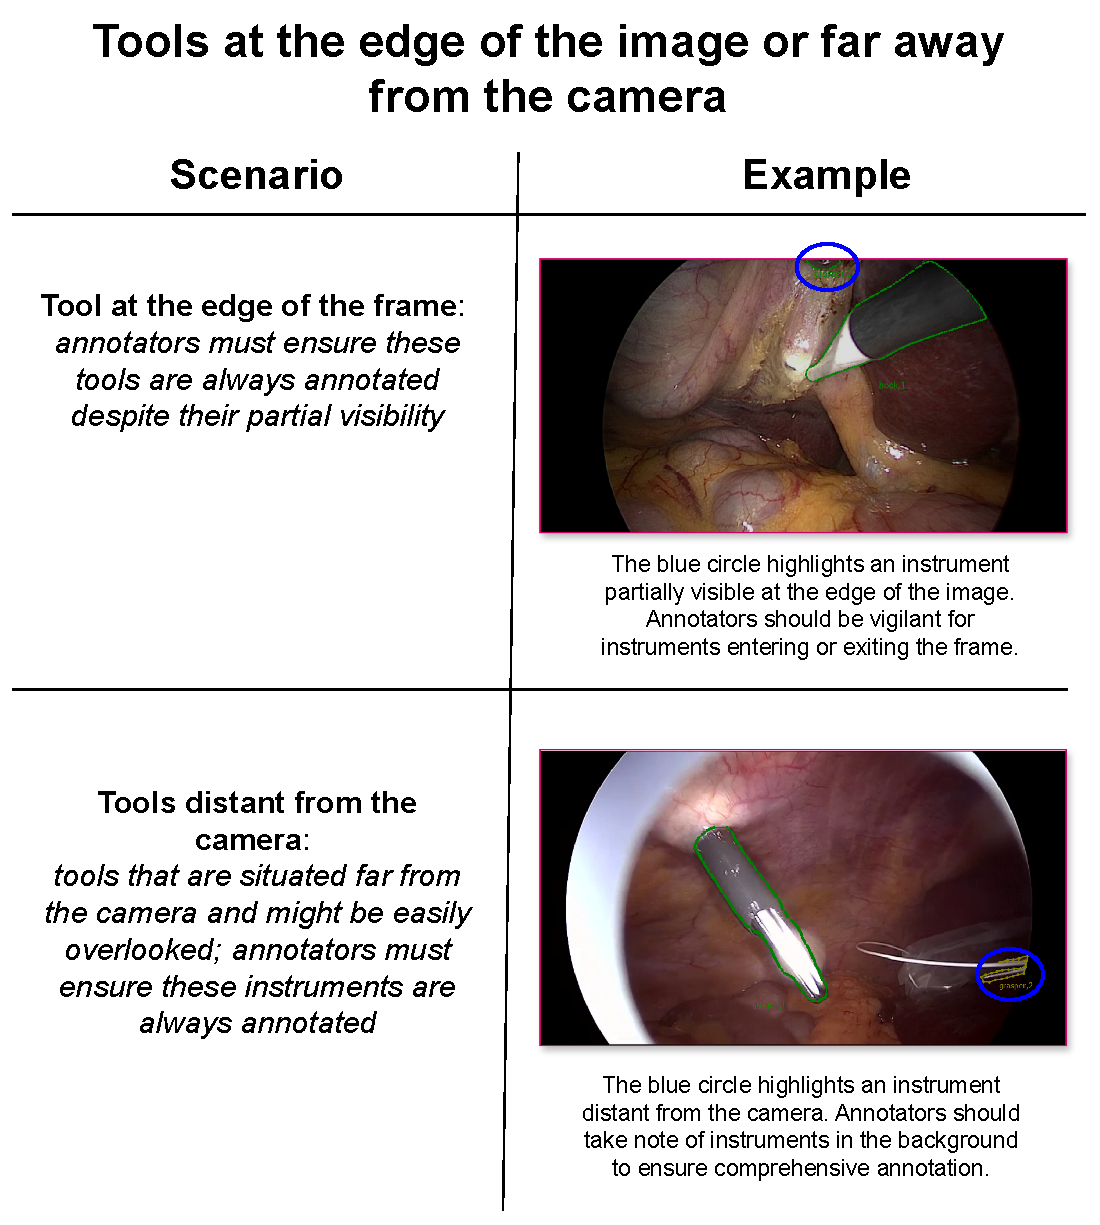
\includegraphics[width=0.9\linewidth]{imgs/hard_cases_far_and_edge.pdf}
  \caption{Annotation guidelines for instruments at the edge of the frame or distant from the camera. }
  \label{fig:edge_distant_tools}
\end{figure}


\begin{figure}[ht]
  \centering
  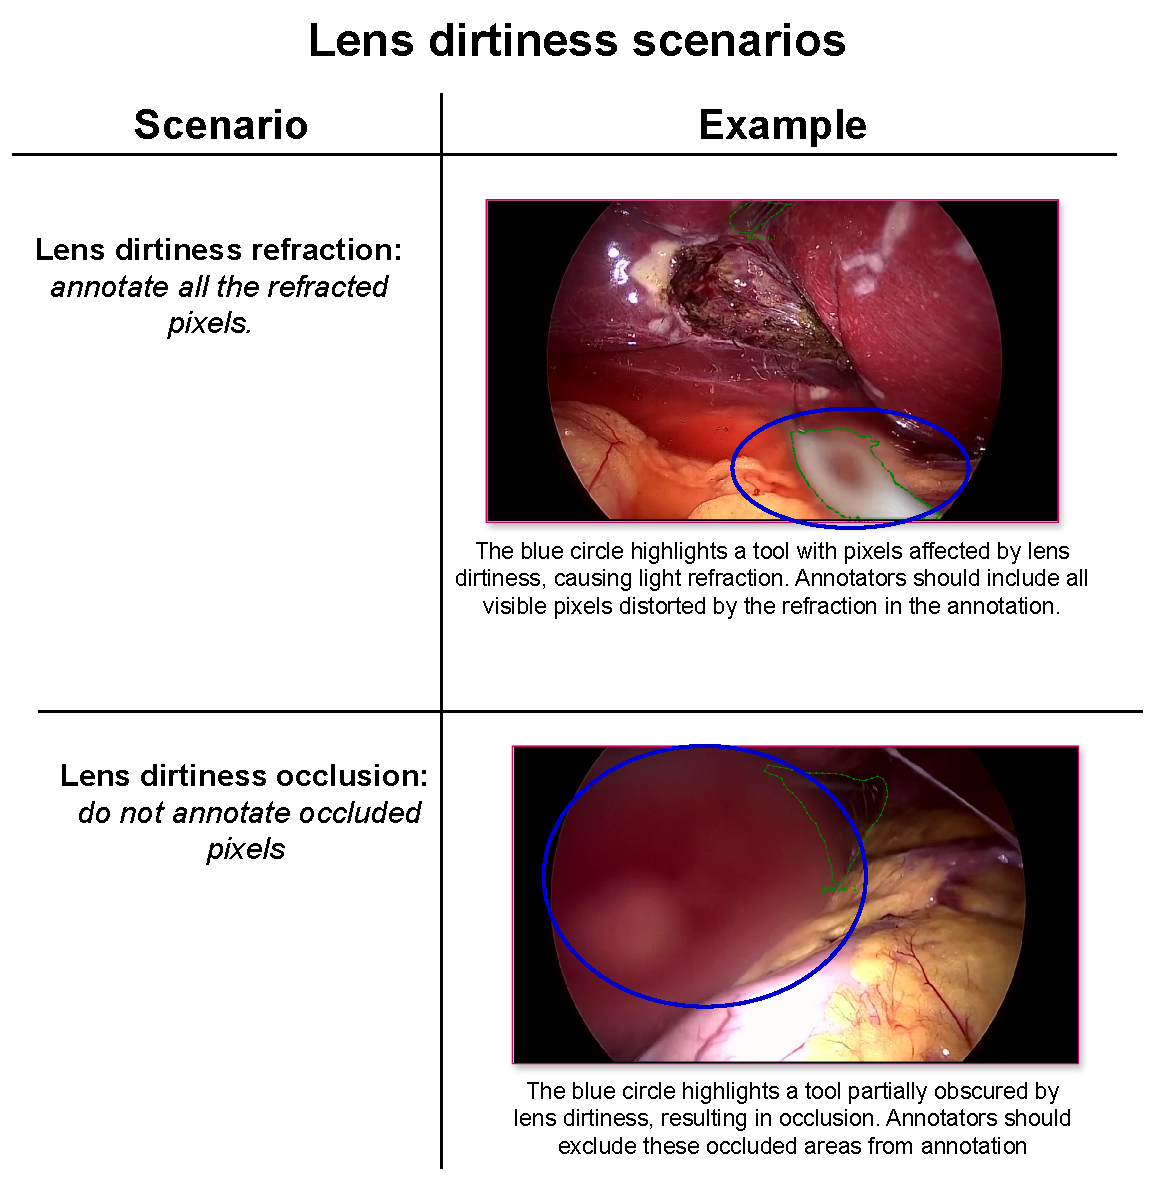
\includegraphics[width=0.9\linewidth]{imgs/hard_cases_lens_dirtiness.pdf}
  \caption{Annotation guidelines for tools affected by lens dirtiness. }
  \label{fig:lens_dirtiness}
\end{figure}


\begin{figure}[ht]
  \centering
  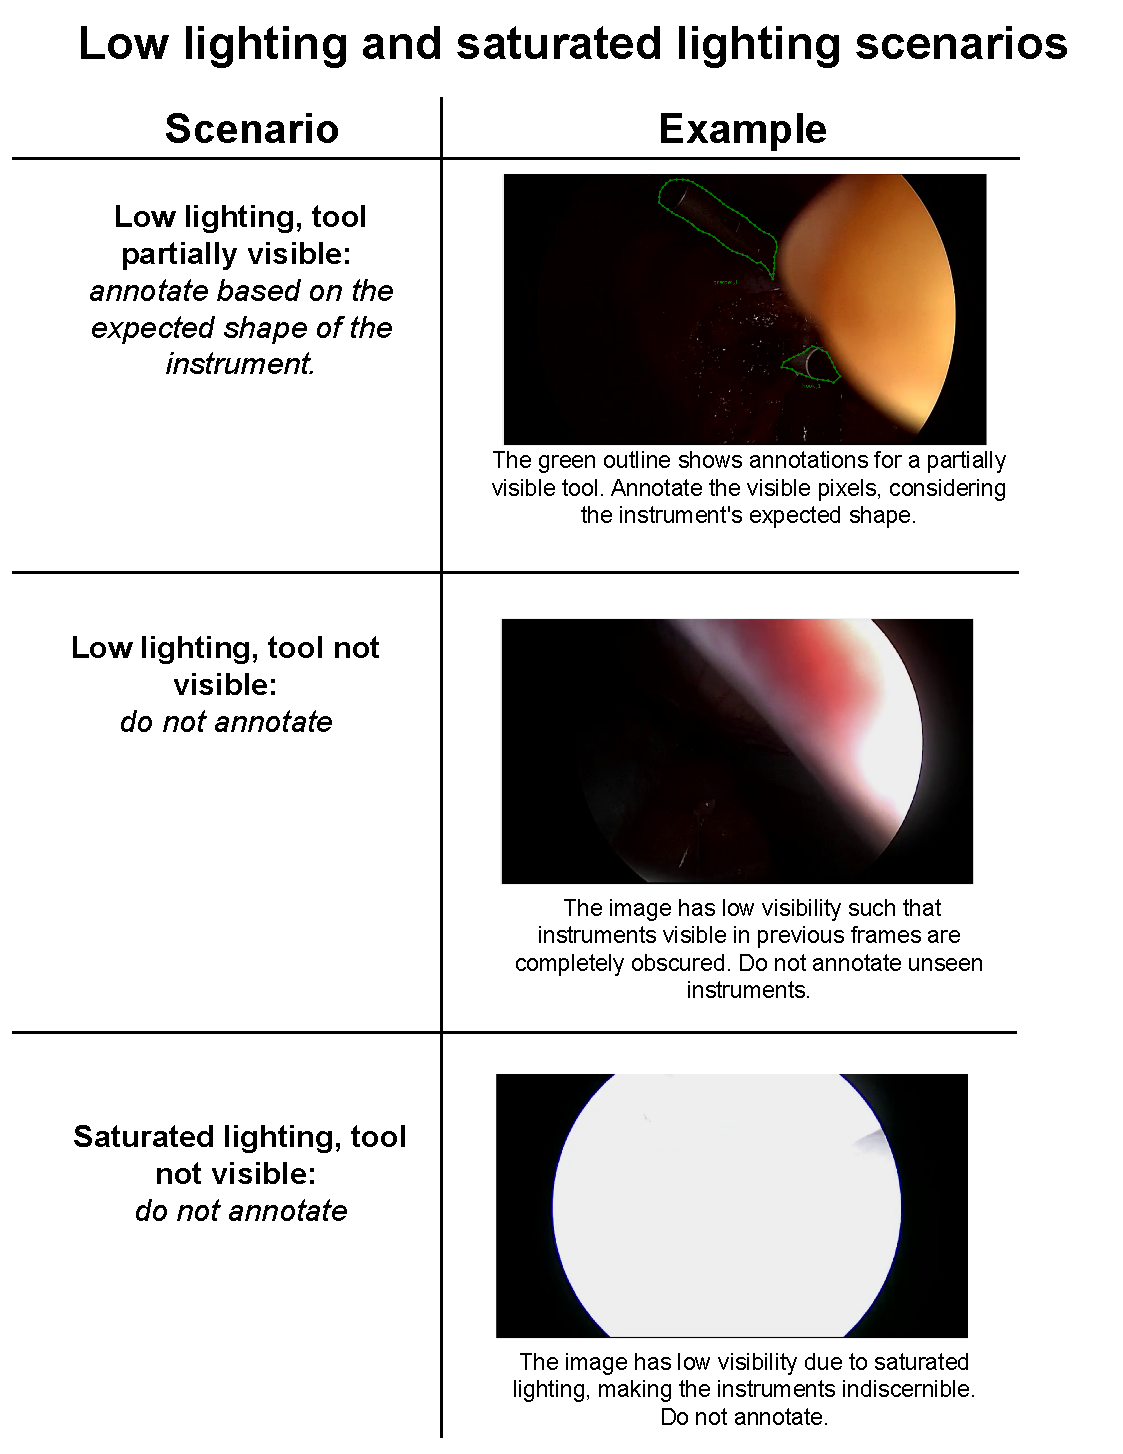
\includegraphics[width=0.9\linewidth]{imgs/hard_cases_low_lighting_and_bright_lighting.pdf}
  \caption{Annotation guidelines for tools in low lighting and saturated lighting. }
  \label{fig:low_lighting_saturated_lighting}
\end{figure}

\begin{figure}[ht]
  \centering
  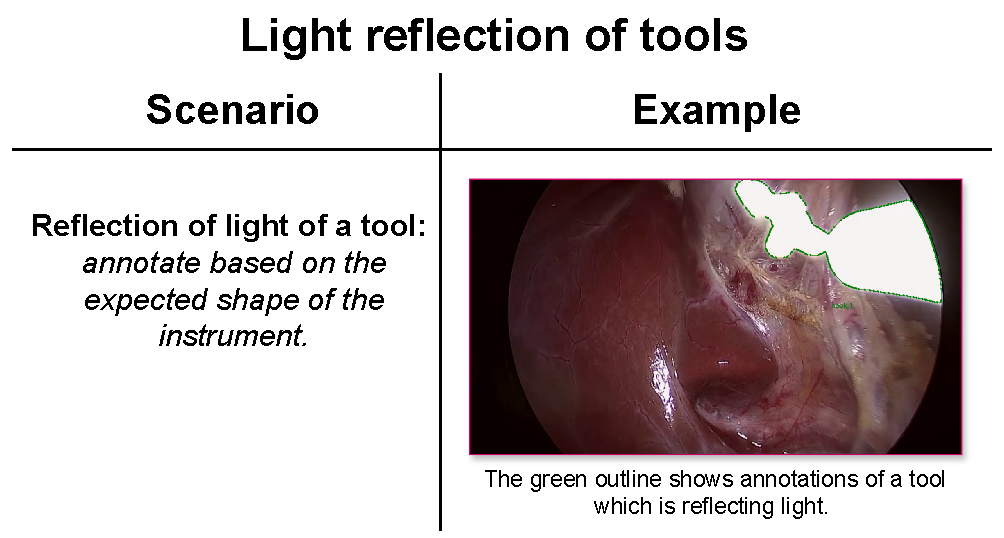
\includegraphics[width=0.9\linewidth]{imgs/hard_cases_reflection.pdf}
  \caption{Guidelines for annotating tools under light reflection conditions.}
  \label{fig:reflection_light}
\end{figure}

\begin{figure}[ht]
  \centering
  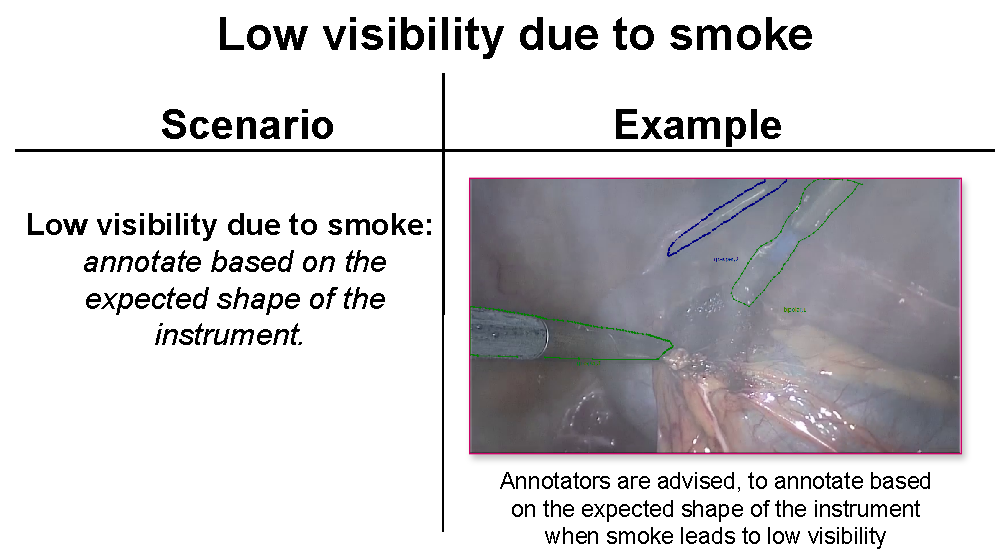
\includegraphics[width=0.9\linewidth]{imgs/hard_cases_smoke.pdf}
  \caption{Guidelines for annotating tools during low visibility due to smoke.}
  \label{fig:smoke}
\end{figure}


\FloatBarrier

\begin{titlepage}
   \vspace*{\stretch{1.0}}
   \begin{center}
      \Large\textbf{More Evaluation metrics for baseline models}
   \end{center}
   \vspace*{\stretch{2.0}}
\end{titlepage}





\end{document}